\begin{frame}{Results on fastSTRUCTURE \citep{raj:2014:faststructure}}

We adapt fastSTRUCTURE
% {\color{blue} \href{https://web.stanford.edu/group/pritchardlab/publications/pdfs/PritchardEtAl00.pdf}{(Pritchard et al. 2000};
% \href{https://www.genetics.org/content/197/2/573}{Raj et al. 2014)}
% },
a Bayesian model for population genetics, to include a BNP prior.


We study genetic data from the Taita thrush, an endangered bird species.
The data consists of microsatellites sequences of 155 individuals at 7 loci.

\begin{figure}[!h]
\centering
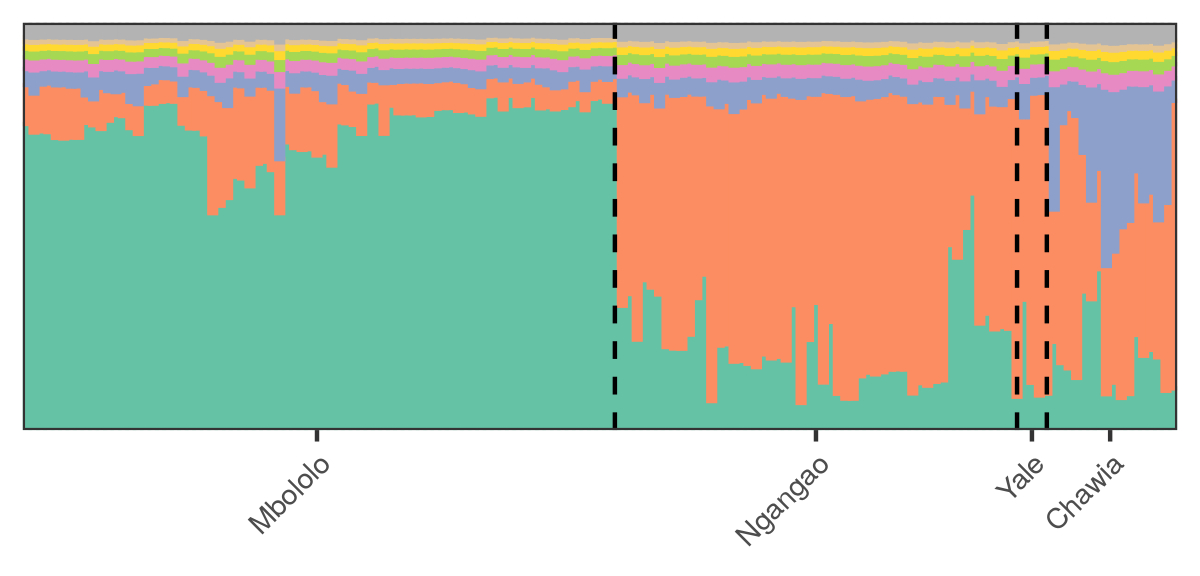
\includegraphics[width = 0.9\textwidth]{./figure/structure_init-1.png}
\caption*{The intitial fit at $\alpha = 3$. }
\end{figure}
\end{frame}


\begin{frame}{fastSTRUCTURE: Parametric Sensitivity}
  \begin{figure}[!h]
    \centering
    \only<1>{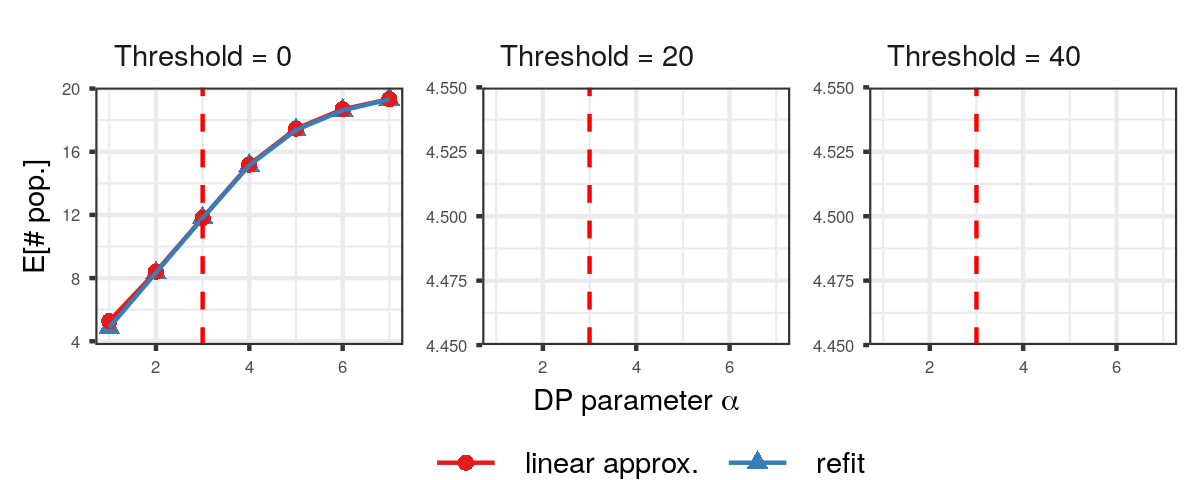
\includegraphics[width = \textwidth]{./figure/structure_alphasens0-1.png}}%
    \only<2>{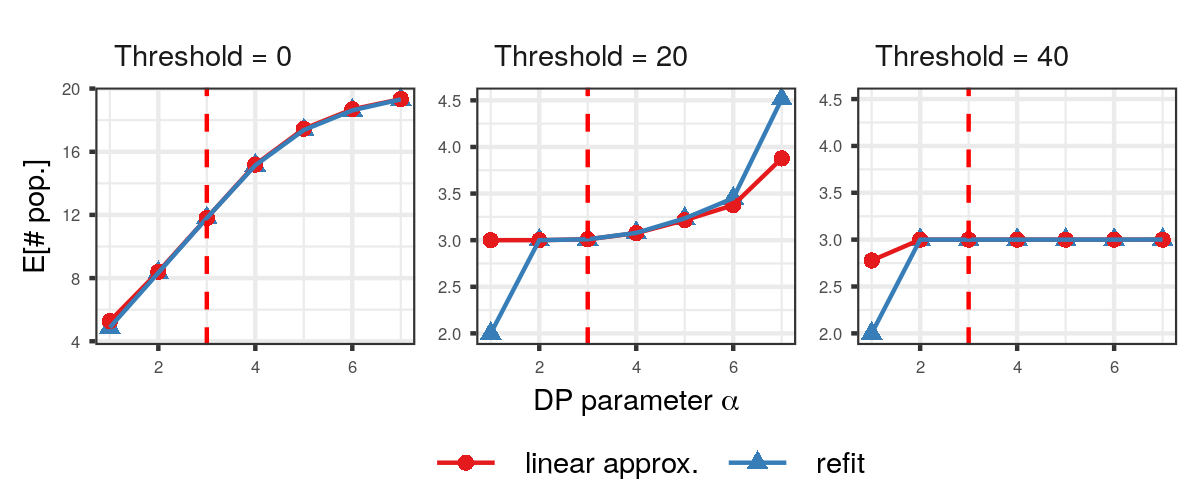
\includegraphics[width = \textwidth]{./figure/structure_alphasens-1.png}}
    \caption*{Expected number of posterior in-sample clusters in the thrush data as $\alpha$ varies.}
  \end{figure}

\end{frame}

\begin{frame}{fastSTRUCTURE: Evidence of Migration?}

  \begin{figure}[!h]
    \centering
    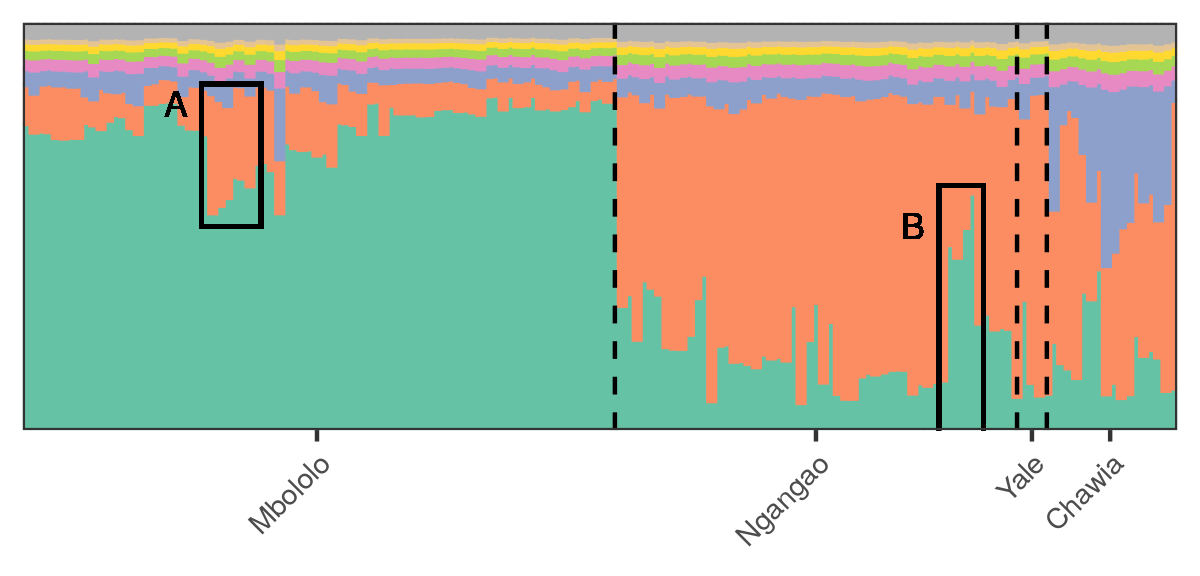
\includegraphics[width = 0.9\textwidth]{./figure/structure_migration-1.png}
  \end{figure}
\end{frame}

\begin{frame}{fastSTRUCTURE: Evidence of Migration?}
    \begin{figure}[!h]
\centering
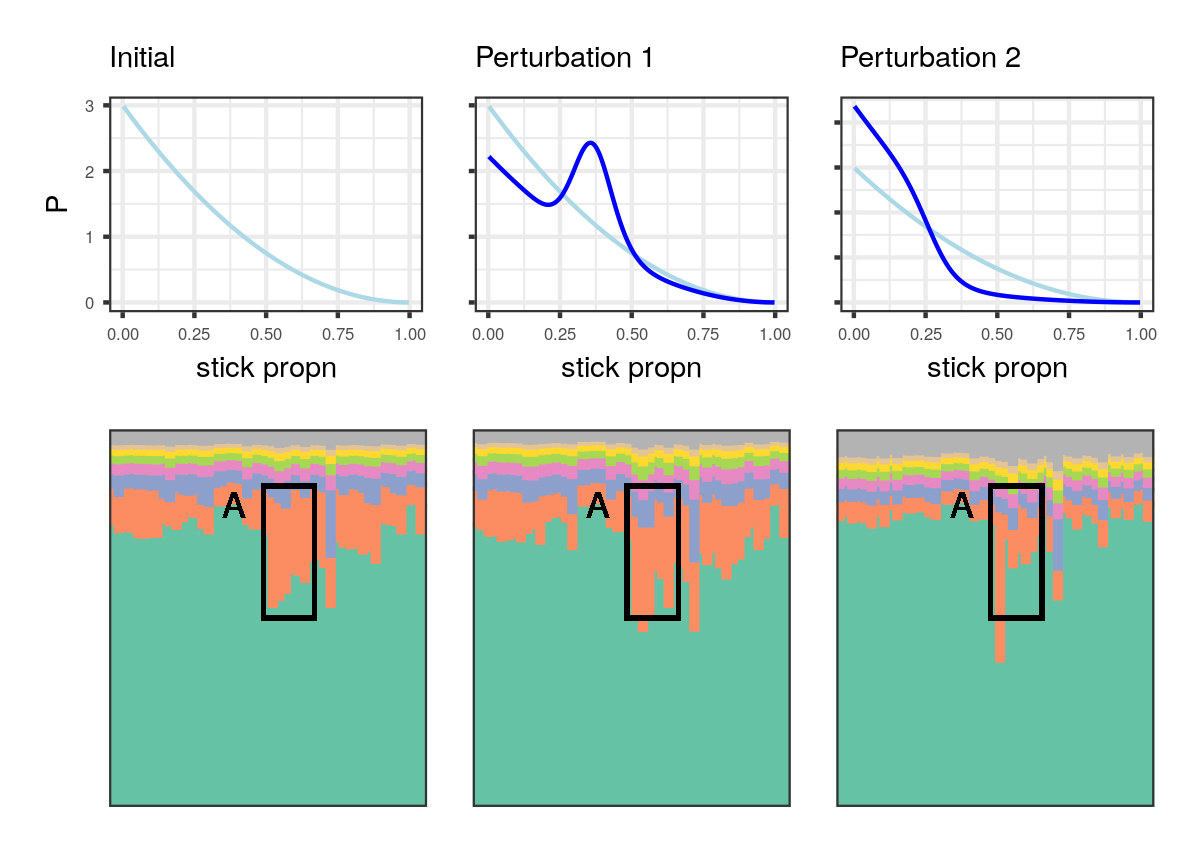
\includegraphics[width = \textwidth]{./figure/mbololo_motivating_ex-1.png}
\end{figure}

\end{frame}

\begin{frame}{fastSTRUCTURE: Functional Sensitivity}

\begin{figure}[!h]
    \centering
    \only<1>{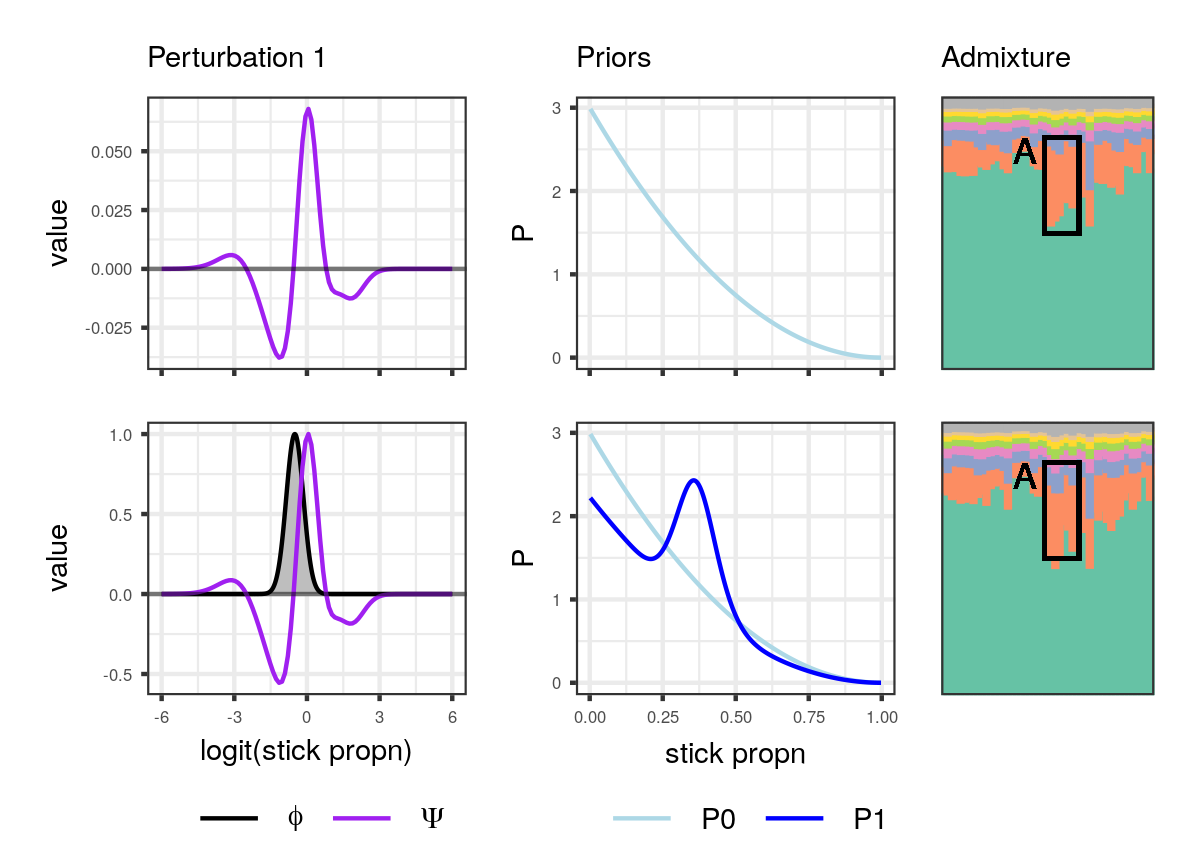
\includegraphics[width = \textwidth]{./figure/mbololo_motivating_ex_inflA-1.png}}
    \only<2>{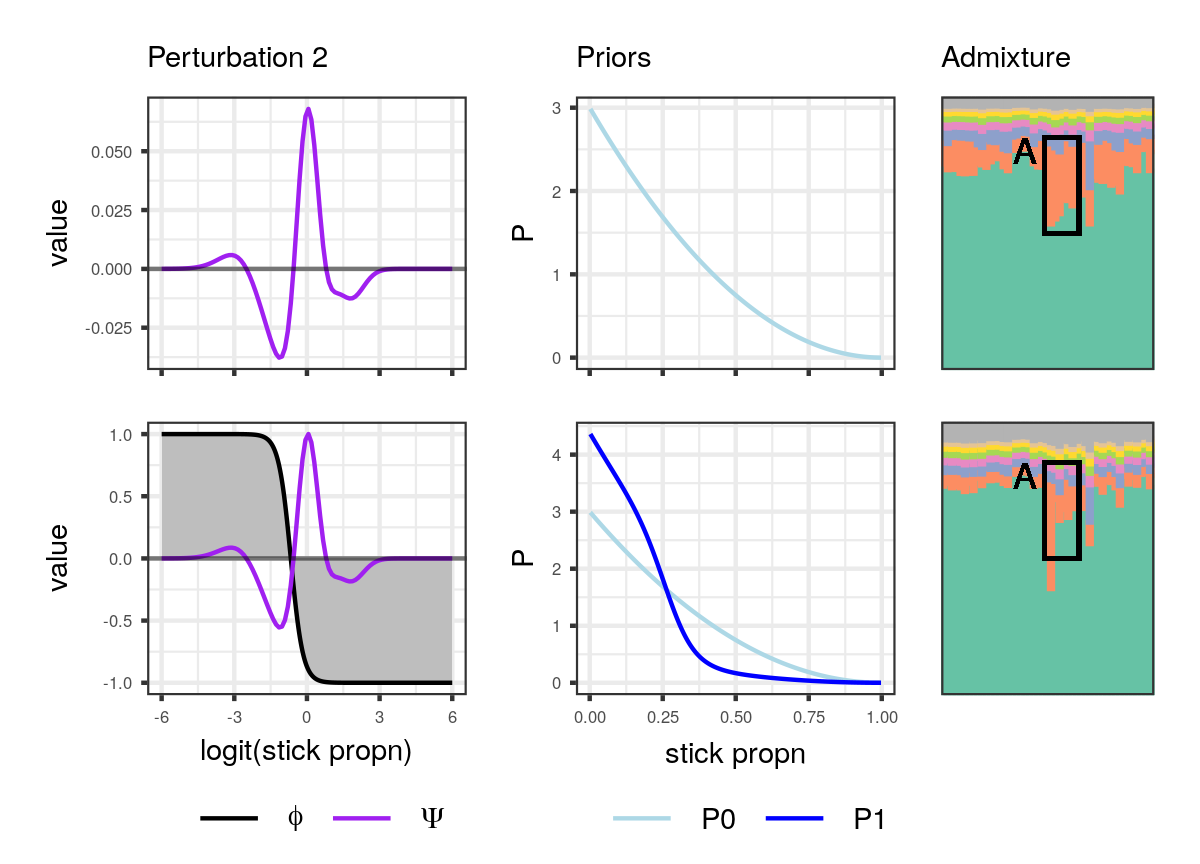
\includegraphics[width = \textwidth]{./figure/mbololo_motivating_ex_inflB-1.png}}
\end{figure}

\end{frame}

\begin{frame}{fastSTRUCTURE: Functional Sensitivity}

  \begin{figure}[!h]
    \centering
    \only<1>{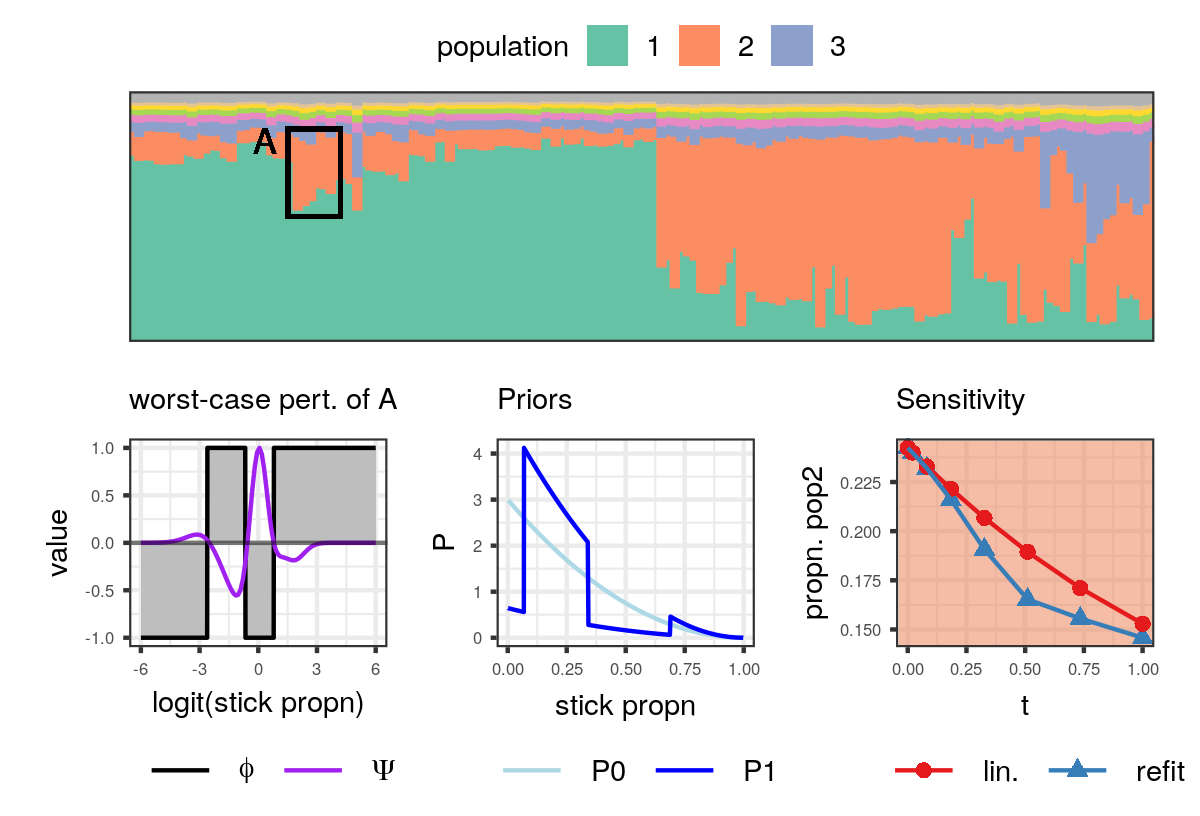
\includegraphics[width = \textwidth]{./figure/mbololo_outliers-1.png}}%
    \only<2>{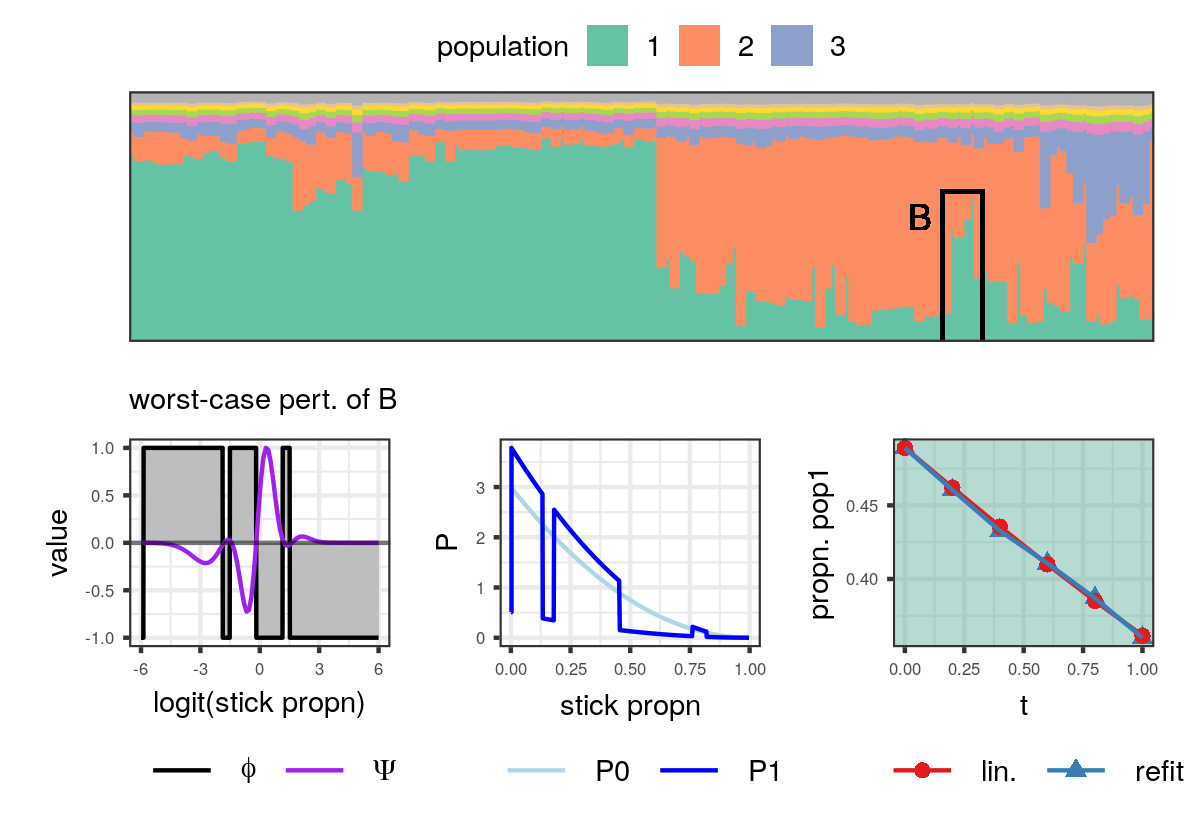
\includegraphics[width = \textwidth]{./figure/ngangao_outliers-1.png}}%
    % \only<3>{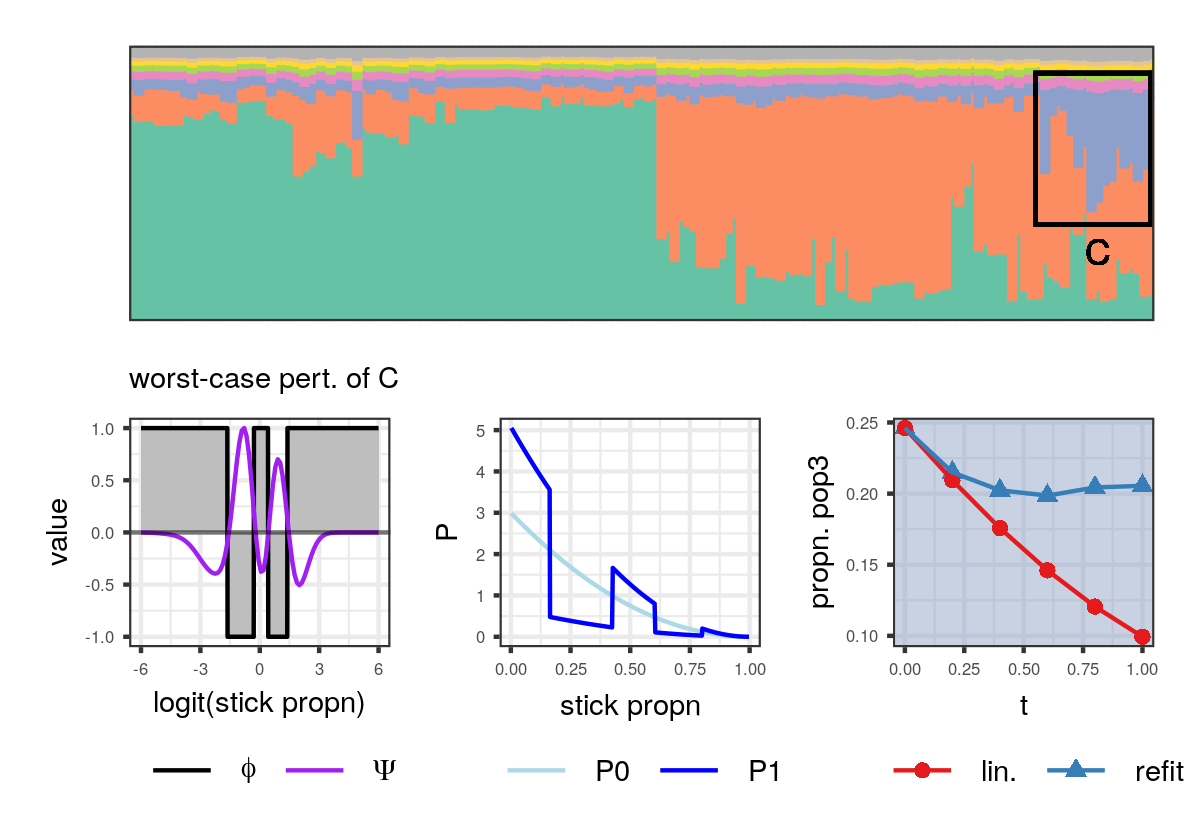
\includegraphics[width = \textwidth]{./figure/chawia_outliers-1.png}}
  \end{figure}

\end{frame}

%%%%%%%%%%%%%%%%%%%
% limitations of local sensitivity
%%%%%%%%%%%%%%%%%%%


\begin{frame}{Limitations of Local Sensitivity}
  \begin{figure}[!h]
    \centering
    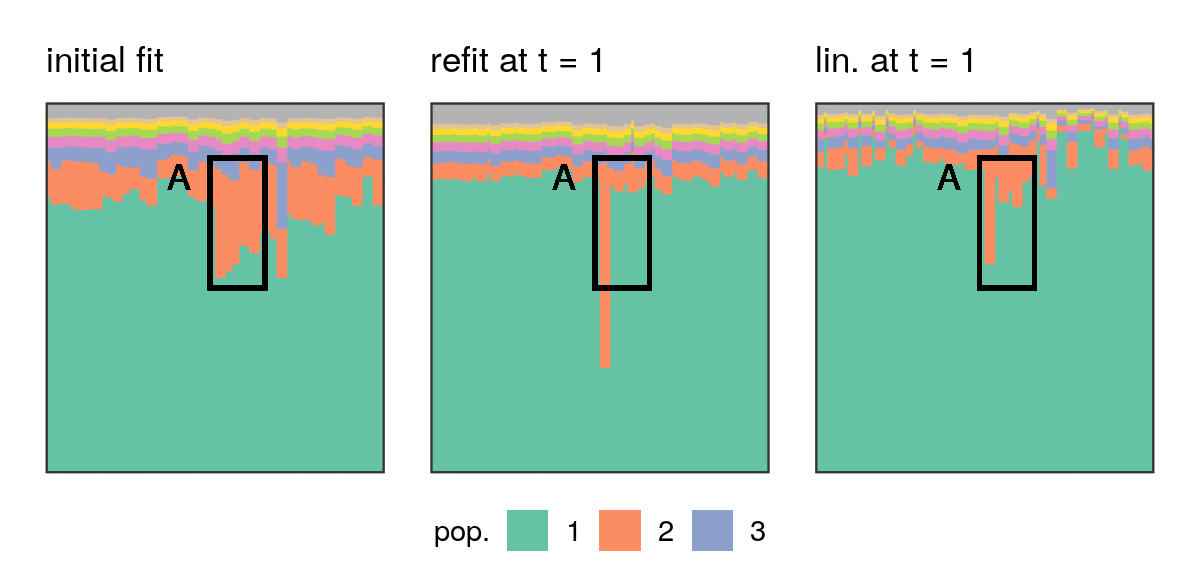
\includegraphics[width = \textwidth]{./figure/bad_admix_ex-1.png}
    \caption*{Inferred admixtures after the worst-case perturbation
     to individuals A.
     Individual $n = 26$ had a large increase in admixture proportion of
     population 2 after the refit. }
  \end{figure}

\end{frame}

\begin{frame}{Limitations of Local Sensitivity}

  \begin{figure}[!h]
    \centering
    \only<1>{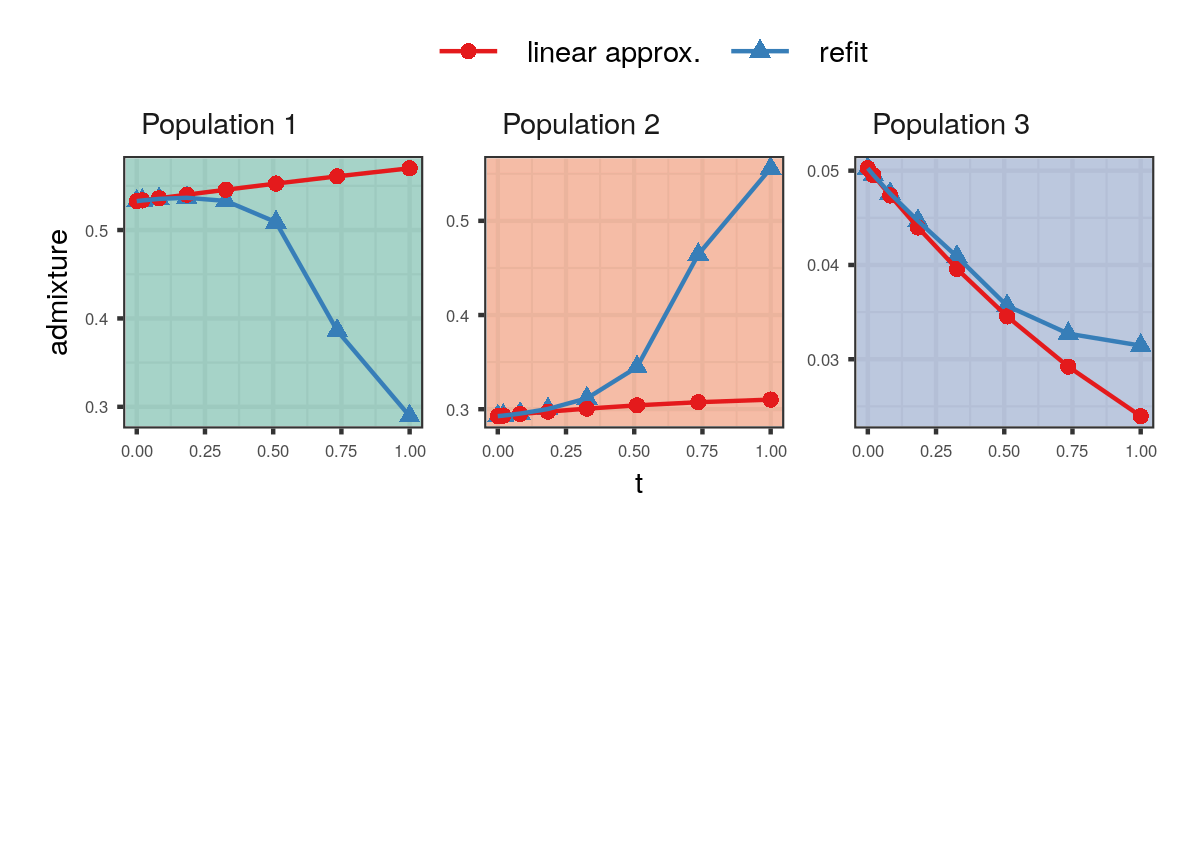
\includegraphics[width = \textwidth]{./figure/bad_admix_trace_admix-1.png}}%
    \only<2>{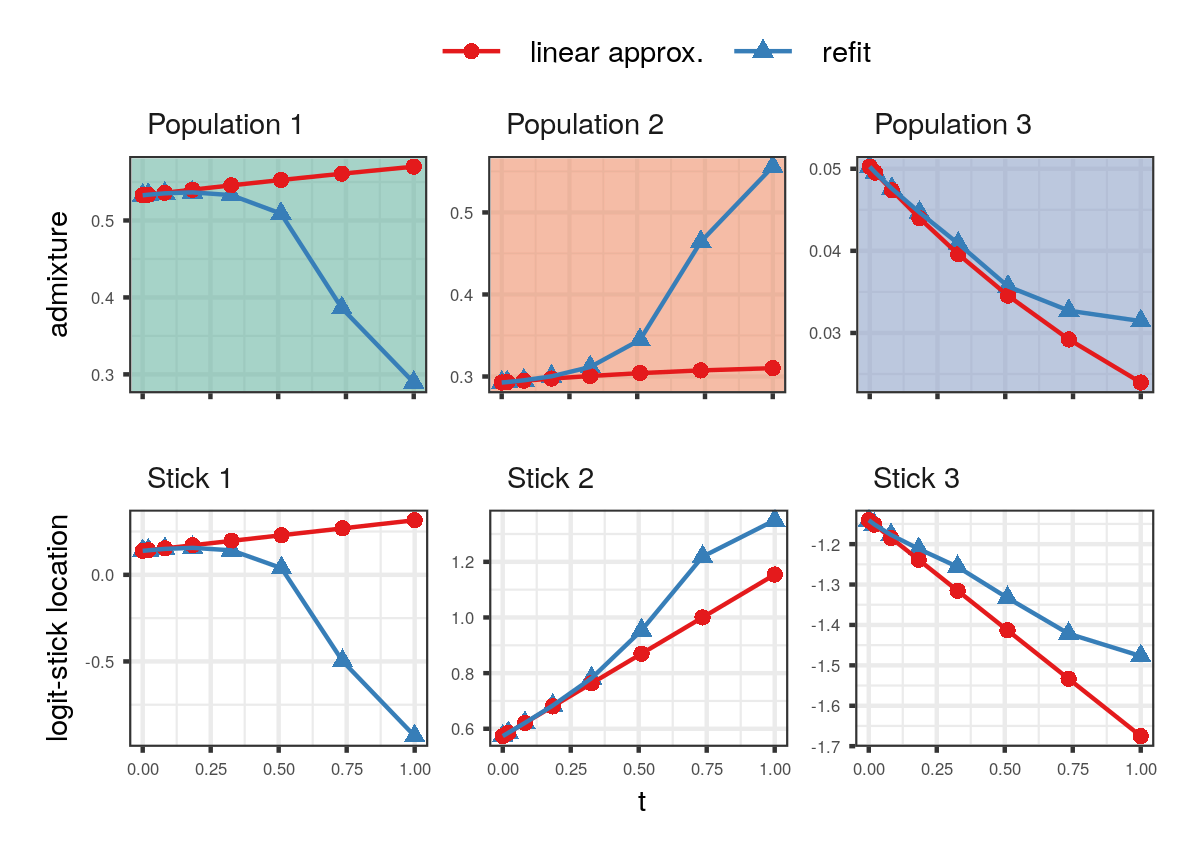
\includegraphics[width = \textwidth]{./figure/bad_admix_trace_all-1.png}}%
  \end{figure}

\end{frame}

\begin{frame}{Computational Complexity}

\begin{table}[tb]
\centering
\caption*{Compute time of results on the Taita thrush dataset. }
\begin{tabular}{|r|r|}
\hline
    & time (seconds) \\
    \hline
    Initial fit & 7 \\
    \hline
    Hessian solve for $\alpha$ sensitivity & 0.3\\
    Linear approx. $\eta^{lin}(\alpha)$ for $\alpha = 1, ..., 7$ &
        0.006 \\
    Refits $\eta(\alpha)$ for $\alpha = 1, ..., 7$ &
        30 \\
    \hline
    The influence function & 0.6 \\
    Hessian solve for perturbation $\phi$ &
        0.4 \\
    Linear approx. $\eta^{lin}(\epsilon)|_{\epsilon = 1}$
      for perturbation $\phi$ &
        0.001\\
    Refit $\eta(\epsilon)|_{\epsilon = 1}$
      for perturbation $\phi$ &
        10 \\
    \hline
\end{tabular}
\end{table}



\end{frame}
